
%2.1
\section{Automatic Identification of Software Bugs}
This section deals with tools that are capable of detecting bugs automatically. We divide bugs in three different categories:
\begin{itemize}
    \item Memory related bugs, e.g. null pointer violation, memory leak and buffer overflow.
    \item Concurrency related bugs, e.g. critical race conditions, deadlock and unsafe concurrent data access.
    \item Semantic related bugs, when the fault arise from a contradiction to the intention of the programmer or the original design.
\end{itemize}
\\
Different tools use different methods to detect bugs; the first big distinction to be made is between dynamic and static analysis.

\emph{Static analysis} is performed with no execution of the program and relies only on the source code or on some object code. 

\emph{Dynamic analysis} executes the program and inspect its behaviour at run-time. It can be implemented in many flavours, for example: with instrumentation of the executable, with a virtual processor or taking the form of a scheduler. Two are the main factors that are often taken under observation, one is the performance loss in the execution and the second is the extension of the run-time monitor (both in quality and quantity).
\\
\\
We can define another distinction on how bugs are identified; many tools use rules to detect if some violation has occurred. The rules themselves are of two types: programming and statistical rules.

\emph{Programming rules} are usually clear and squared, e.g. they derive from axioms, mathematical models or are manually defined.

\emph{Statistical rules} are defined through a statistical analysis on multiple samples. Usually there is a training phase where observations are collected and correct rules (invariants) are refined.
\\
\\
Another means of detecting bugs is \emph{model checking} where the tool verify correctness in a usually finite state system. This verification is performed using formal methods on typically formally specified system. 

The last category for bugs finding techniques is the \emph{annotation-based} tools. Those requires the annotation of programs to extract semantics and verify consistency and correctness.
\\
\\
What follows is the description for each selected tool.
\\% 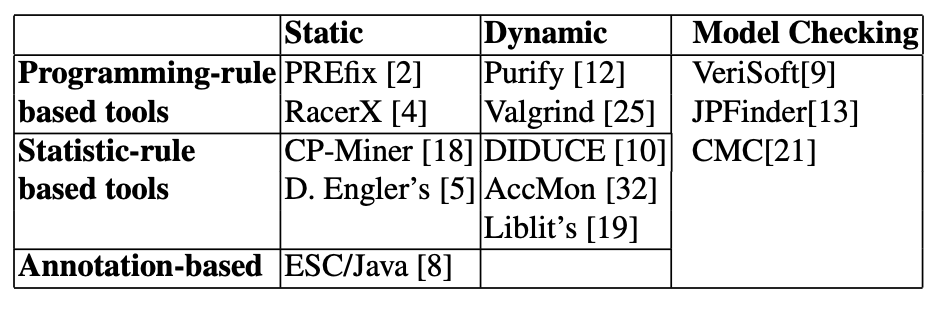
\includegraphics{classification-of-bug-detection-tools.png}
\\
\labeltextbf[]{PREfix}{bug:PREfix} \cite{bush2000static} A static analyzer for finding dynamic programming errors

PREFix is a source code analyzer that detects a broad range of errors in C and C++ code.
Its goal is to detect many runtime issues on real world programs, without dynamic analysis and instrumentation; only the source code text is used. PREfix can detect defects efficiently through a model that abstracts functions and their interactions; the analyzer traces execution paths handling multiple language features: pointers, arrays, structs, bit field operations, control flows statements and so on.

The method used by the tool is based on the simulation of individual functions. It employs a virtual machine that simulates the actions of each operator and function call. With the detailed tracking it can report defects information to the user so to easily characterize the detected error.
The tool can be applied both to a complete program source or only a subset. This bottom up approach is particularly useful when the source code is not fully available (e.g. in the case of a thirty part library).
\\
\\
\labeltextbf[]{RacerX}{bug:RacerX} \cite{engler2003racerx} RacerX: effective, static detection of race conditions and deadlocks

RacerX deals with complex multithread systems. It detects race conditions and deadlock using static analysis.
It can infer from the source code the object lock that is assigned to a particular code block. It detects code that is used in a multi-threaded context; it also detects when the code endeavours in dangerous shared access. 

RaceX uses annotations only to mark the code that deals with lock acquisition; this requirement keeps the burden on the user to the minimum to increase ease of adoption. The authors of RaceX report their experiences on the biggest problem about race detection: in large codebase there are massive amounts of unprotected variable access; the key point is to report only those that can actually cause problems. There is emphasis on two aspects:
\begin{itemize}
    \item The first is to minimize the impact of reporting false positive in order to avoid the users to discard the use of the tool; to achieve this, RaceX employs specific techniques to lower the impact of analysis mistakes.
    \item The second is the speed of the tool: the authors keep the time of execution for the analysis under deep scrutiny; they claim that for a codebase of 1.8 LOC the time required is between 2-14 minutes.  
\end{itemize}
\\
The tool has been found capable of finding severe problems in huge projects like Linux, FreeBSD and also in a large closed source commercial software.
\\
\\
\textbf{Purify} \cite{hastings1992fast} Fast Detection of Memory Leaks and Access Errors. Winter 1992 USENIX Conference
 
 Purify is a dynamic analysis tool for software testing and quality assurance . 
 It instruments the object files generated by the compiler (the software dates back to 1992 and the supported platform is Sun Microsystem's SPARC); the process that acts on the object files  include also third-party libraries. 
 Purify detects multiple errors: memory leaks, access error, reading uninitialized memory. The injected instructions check every read and write memory operations; the slow down of the target is under three times in respect to the non-instrumented execution time. 
 Enabling the use of Purify is as simple as adding a word in the makefile; the generated overhead is inside the limit of tolerance of developers and it allows to detect bugs early in the development cycle.
\\
\\
\textbf{Valgrind} \cite{nethercote2007valgrind} Valgrind: a framework for heavyweight dynamic binary instrumentation

Valgrind is a framework available for many Linux, Android and Darwin architecture. 
It is the foundation where many tools are built upon. All these tools, several are already included with the standard distribution, help to build more correct and faster program and are categorized as dynamic analysis tools.\\
The eight supplied tools can be divided in the following groups: memory error detector, cache profiler, thread error detector, heap profiler.
There are also two additional tools that are provided to illustrate how to use the framework works and how to use the core low level infrastructure to implement instrumentation.
\\ 
Basically, the core implements a synthetic CPU that asks the selected tool how to instrument the code and then continues and coordinates the execution. All the instructions are simulated and the memory access is sandboxed; this includes also the third party library linked into the executable. There are ways to manage and suppress every output generated to avoid clutter and unwanted error reports.
\\
It is advised to enable the debug info into the executable; without them Valgrind is unable to determine which function is the owner of a specific instruction, as such it will produce almost useless error and profiling messages. It is also advised to use minimal compiler optimization to avoid incurring into false positive error reports.
\\
The slowdown of the execution depends on the specific instrumentation of the selected tool, and it is roughly between four to fifty times of the original speed. 
%EXPAND% The most popular tool in the suite is Memcheck; 
\\
\\
\labeltextbf[]{CP-Miner}{bug:CP-Miner} \cite{li2006cp} CP-Miner: Finding Copy-Paste and Related Bugs in Large-Scale Software Code

CP-Miner stands for Copy and Pasted code Miner. Zhenmin et al. found that a significant portion of source code in many widely used open source projects are duplication made with copy and paste. This practice introduces bugs, the main reason being that programmers leave identifier untouched instead of renaming them consistently to match the new code context. When the label do not exists in the new place it will be detected with a compilation error; on the other hand, if the identifier exists in the new context it will not be detected by the compiler and it will introduce a hidden bug very hard to detect.\\
CP-Miner tolerates modification to the pasted code. In order to be detected, the segments do not need to be identical; they can also contain insertions or modifications. The tool is capable of detecting duplicated code but not all detection are true positive; nonetheless it is able to report many significant duplicates with hidden issues. The authors detected 28 copy-paste related bugs in the Linux kernel code base and 23 in FreeBSD; these bugs were reported and most of them where previously unknown to the project team.
The analysis is done infra-project and targeted the following large projects: Linux, FreeBSD, PostgreSQL and Apache HTTP server.
\\
The main contributions of the paper are: scalability, bugs detection and statistical study of the copy-pasted code. 
\begin{itemize}
    \item \emph{Scalability} is a strong point of CP-Miner because the technique used in it allow to quickly and efficiently scan large projects including operating system code. For example, it took 20 minutes to find 150,000-190,000 copy-pasted segments respectively in the FreeBSD and Linux kernel; such fragments account for roughly one fifth of the code base. At the time, both projects had more the three million lines of code. 
    \item \emph{Bugs detection} was found to be very effective because of the positive response from the open source project maintainers; most of the reported bugs were not found by static or dynamic analysis detection tools. 
    \item The authors conducted a \emph{statistical study} of the copy-pasted code to give an overview of the phenomenon; the majority of the copied code is between 5 and 16 statements. Around 50 percent of the code has only two copies but around 7 percent has more than eight duplicates. Roughly 12 percent of the copy-pasted code segments are whole functions. Kernel modules are affected with different concentration, depending on the module under analysis: drivers, arch and crypt modules have high copy and paste segments than other parts of the project.
\end{itemize}
\\
\\
\textbf{D. Engler's} \cite{engler2001bugs} Bugs as Deviant Behaviour: A General Approach to Inferring Errors in Systems Code

The approach taken by Engler et al is to extract from source code beliefs and properties that must or could hold. Through static analysis it is automatically detected two different types of beliefs: MUST beliefs and MAY beliefs. The first one is something that must certainly hold, for example the dereference of a pointer holds the credence that the reference is not null and must be valid. The second one is statistical by nature; the code is observed and searched for patterns that suggests beliefs, for example a call to function "x" followed by a call to function "y". The probabilistic nature of the MAY belief comes when validating it: at first it is treated as a MUST belief then a search yields all uses in the source code of such belief (i.e. the use of "x" and "y"). If it turns out that such pattern is respected most of the times then the belief is probably valid, otherwise it is treated as a coincidence and, as such, discarded.
MUST beliefs bear no doubt about their validity and represent internal consistency. All contradictions from both MUST beliefs and valid MAY beliefs are reported as errors (i.e. bugs).
The authors leverage their prior work \cite{engler2000checking} where they used static analysis to fix manual defined rules for specific system; for example a call to spin\_lock(l) must be paired with a following spin\_unlock(l). Such patterns were previously specified by hand; with the current work they enable a system to infer the same (and more) rules automatically. They reported that the automatic system is able to detect all the manual rules plus a considerable additional amount that goes from ten to one hundred patterns more.
The general idea underling this paper, is that the source code contains intrinsic information about what is correct; finding errors in real system means exploiting what is intended as "correct". Sadly, most of the times these rules are not documented, not formalized or if they are available, they are present in informal and unusable format.
With this work the authors use static analysis to extract the beliefs that the programmers infused in the source code, without the need of a priori knowledge.
Manually performing the task of extracting correct behaviours and rules from source code is usually a hard, difficult and daunting experience, particularly in view of multiple releases and big code bases. Engler et al show of being able to apply this techniques to complex systems as Linux and OpenBSD operating systems. The results are hundreds of detected contradictions (i.e. errors or bugs) reported; many of them have been assessed and resulted in kernel patches.
\\
\\
\textbf{DIDUCE} \cite{hangal2002tracking} Tracking Down Software Bugs Using Automatic Anomaly Detection

The paper introduces a tool written by the authors called DIDUCE: Dynamic Invariant Detection $\cup$ Checking Engine.
It is based on instrumentation of Java programs so to observe their behaviour at run-time. During the lifetime of the target Java process, DIDUCE gather information and collects hypothesis of invariants; those are the rules that the program should obey. As violation to the invariants are encountered the tool relaxes the hypothesis allowing for different behaviour. Every invariant has a confidence level, the process previously described updates it; then the user can go through all the anomalies reported ordered by their rank. The tool is intended to be used in the discovery of the root cause of bugs and as an aid in better understanding the program under analysis. 
The query of this ranking can be done, for example, just before a crash occurs: inspecting what DIDUCE detects as anomalies often lead to the discovery of the root cause of the problem.

The paper describes also the findings during the application of DIDUCE to four Java real-life programs, one of which is the JSSE Library (Java Secure Sockets Extension); the bug under analysis was found during the development of a proxy server to be applied to the JSSE Library. The problem was that using the proxy server triggered unexpected behaviour in the JSSE internals. Thanks to DIDUCE the programmer was able to find the issue in the core of the library: it was reported with high confidence that method read() returned a different value than usual. This method returns the number of bytes read from the stream and Java specs clearly define that the method can also return with a buffer not fully filled. A common Java programmers pitfall is to ignore this result and skip the loop on read() to obtain all expected data. DIDUCE reported a violated invariant with high confidence because the result from the method was always 74 and in one instance (just before the Exception) the number was smaller; this information made apparent that using the proxy triggered a bug present in JSSE Library.
The authors' experience suggests that discovering bugs using their proposed methodology is simple across many different kind of programs, shown in the paper with four compelling cases.
%expand the idea of "DIDUCE, what's new? what changed up to a point?"
\\
\\
\textbf{AccMon} \cite{zhou2004accmon} AccMon: Automatically Detecting Memory-related Bugs via Program Counter-based Invariants

The contributions of this paper are two innovative ideas: the first is a novel statistical approach to detect bugs in memory related issues, the second is a novel architectural extension to decrease the overhead of the monitoring process.

The first is called PC-based invariant detection (PC stands for program counter); it leverages the observation that most programs access memory location mostly from the same instructions. Being probabilistic in nature, it can detect memory access anomalies that deviate from the baseline; they usually are the causes for bugs, stack overflows and many other memory-related issues. We can see that there are tho phases: one where the statistical data are gathered and the baseline rules (e.g. invariants) are formed; the other phase put to use the collected rules and check for violations that will be reported.
These two phases are intended to be used in multiple runs but also in the same single long-running execution.


The second contribution is called Check Look-aside Buffer (CLB); it aims to lower the burden of the dynamic process monitor activities to decrease the overhead needed. The authors report their experiments on performance: in the worst case analyzed the loss of speed of the process is less than 3 times. In other tools, this slowdown can be of one order of magnitude greater.

The effectiveness of the authors' contribution are tested through AccMon, a tool they developed in order to implement the idea of a PC-based invariant detection; such experiments shows that the proposed novel ideas are sometime capable of finding more bugs in respect to other tools such as Purify or CCured. Then, in conjunction with previous work from the same authors (iWatcher) it is demonstrated the effectiveness of CLB in lowering the burden of the overhead.

The authors report many other advantages in using AccMon in respect to other tools:
\begin{itemize} 
%\itemsep0em
\item the analysis is not done on the values of the variables, thus It can detect also bugs that do not violate value-based invariants.
\item in the current form, it uses source code to achieve compiler-based optimization but it can directly work with binaries without the need of compilation.
\item it does not need type information; given it's statistical nature it can detect anomalies just using abstract memory pointers.
\item it's possible to switch off the monitoring activities dynamically at runtime, with almost no overhead. The authors states that AccMon can be used in production runs.
\end{itemize}


\noindent \textbf{Liblit's} \cite{liblit2003bug} Bug isolation via remote program sampling

The underling observation that pave the road for this paper is that often the user community of a program has more raw throughput of running and executing it than the developers. In other words, the number of executions that the team responsible for the program can apply for testing is dwarfed by the number of executions that the community can or will bring up to bear.
The authors propose an infrastructure for gathering data from the user's execution to a central information store; then they propose a process, called automatic bug isolation, to analyze gathered data in order to provide information to the developers to help find and fix bugs.
This infrastructure shows multiple benefits:

\begin{itemize} 
\item Use a vast amount of data that is generated by the execution of the program by the user community; it is usually discarded and do not contribute to better the quality and the experience for the user itself.
\item Enabling the collection of information helps to draw a clearer picture on the effective use of the program and drive better decisions about development roadmap
\item Map and define feature usage statistics
\item Avoid issues related to manual feedback generated from an user intervention: usually the user is unsophisticated and non technical; it's ability to have a positive impact on the bug reporting is limited. The benefits of automatically gather this information are many and varied.
\end{itemize}

Designing an infrastructure that was able to scale was a non-trivial process; there are two main issues to address.

One is to make the lowest impact on the performance on the program execution. It is very important to be respectful of the resources used in gathering debug information. To achieve this goal, the authors employ sampling; they also address a technique to conduct fair sampling.

The other one is a craftiness in gathering and periodically sending data to the central system: even collecting a small amount of information have an huge impact on scalability.

The authors then focus on the data analysis phase. They propose three different application with increasing level of sophistication:

\begin{itemize}
    \item They show how to share the burden of assertion across the use base so to inflict upon each user only a small fraction of the checks.
    \item They show how to start from a large set of predicates (predicate guessing) and shrinking it down over time to reveal the smallest set that can deterministically predict a bug.
    \item They show how to use linear regression to isolate non-deterministc bugs; in other words they shrink the set of predicates that has the highest correlation with the failure.
\end{itemize}
\\
\\
\textbf{ESC/Java} \cite{flanagan2002extended} Extended Static Checking for Java

This tool perform static analysis on Java source code looking for errors and warnings to report. It provides specific Java annotation to formally express design decisions. 
ESC handles and warns about multiple common programming errors, e.g. null dereference, index out of bounds, types errors; it also warns about concurrency errors, like race conditions and deadlock.
Aided by the custom annotations, ESC employs an engine to decode the semantics of the program and apply techniques to automatically prove theorems; doing so it is able to report potential bugs that are not detected by the type system and that are detected at runtime.


One core requirement imposed on ESC is the modularity of checking; in other words, it can work on pieces of code (i.e. methods) in isolation to the rest of the code. This restriction was chosen for scalability reasons even if the downside is the need of custom annotations.
The authors argue that the cost of using the annotations are not an hard overhead: when developers are engaged in manual code review they need information that usually come from unstructured sources (e.g. natural language comments) and they already sustains the burden of gathering additional knowledge not present in the raw code.

It is evident throughout all the paper the importance the authors put on the tradeoff between the cost of the annnotation process and the benefit of true errors feedback; this sentence taken from the paper's introduction sums the core of this tradeoff: "if the checker finds enough errors to repay the cost of running it and studying its output, then the checker will be cost-effective, and a success".
Infact, they enumerates two important features needed by an ideal static checker : 
\begin{itemize}
    \item soundness - if the program has errors, it will find some
    \item completeness - every error reported is a true positive
\end{itemize}
ESC do not seek to honor these two features for the very belief quoted above. The authors observe that the alternative processes used to achieve software quality (testing and code reviews) do not possess any of the features of the ideal static checker.

At paper time of writing, ESC was used for two years on multiple kind of programs and was proven effective in finding meaningful bugs. The performance was adequate for interactive use on most methods. 
Even if it was proven of real usefulness, the users' feedback suggest that the cost of annotating was high and the number of warnings was excessive.
It must be said that the annotation were added after the development of the project and not during the evolution of it; this is commonly know by developers to be a dreaded task. 
\\
At this point it is unclear if the tool delivers a positive tradeoff between cost and benefit; the experience of the authors during internal use of the tool was encouraging. They believe that ESC is already a valid tool to be used in classrooms: it enforces good design, modularity and verification.
\\
\\
\textbf{VeriSoft} \cite{godefroid1998model} Model checking without a model: An analysis of the heart-beat monitor of a telephone switch using VeriSoft

The goal of VeriSoft is to detect problems in a concurrent reactive system (CRS) through the exploration of its state space. The \emph{reactive} word stands to describe the continuous interaction of the system with the environment.
The issues detected are: deadlocks, assert violations, livelocks. 
A CRS is composed of two parts: a finite number of processes written in arbitrary code (e.g. C, C++, Java, tcl, and so on) and a finite number of communication objects (TCP connections, semaphores, shared memory, and so on).
The need of such tool arise from the difficulty of writing a robust and reliable CRS; it is well accepted that concurrent systems are prone to unexpected issues, difficult to track, test and to reproduce.

What VeriSoft does is a systematic state space exploration; it defines the state space as a directed graph: the nodes are the global states and the edges are the transitions between states. 
It follows that each global state should be uniquely identified and this is one of the core issue that VeriSoft solves with an original combination of algorithms; the author calls it "an efficient state-less search".

The paper reports the analysis conducted with VeriSoft on a software owned by Lucent Technologies: "Heart-Beat Monitor" (HBM). Such software monitors the status of a telephone switch elements and determines their state based on the propagation delays of messages sent through those elements.
HBM is an important piece of software because it has a big impact on the switch performance due to its influence on the switch routing.

The experience of the authors is reported as successful: they were able to find errors in the documentation and in the software itself. Subsequently they modified the code to strengthen some properties and tested them again with VeriSoft; after another run, as desired, VeriSoft reported satisfactory results.
The development team of HBM decided to integrate the code changes from the authors for the next commercial release.

VeriSoft acts as a scheduler and has complete control over non-determinism so it can reproduce any interesting scenario (i.e. those that during the automatic tests led to errors and issues).
One other benefit is that there is no need to describe the model with specific languages: it relies on the exercise of the actual code.
One downside is that it cannot detect cycles in the graph of the global spaces and, as such, it can only detect violation of safety properties.
\\
\\
\textbf{JPFinder} \cite{havelund1999applying} Applying Model Checking in Java Verification

Java PathFinder (Jpf) is a prototype translator from the Java language to Promela (Process Meta Language). Promela runs on SPIN (Simple Promela Interpreter).
SPIN is a general tool to find concurrency problems and verify the correctness of a system.

It is reported that Jpf is not the first attempt of Java-to-Promela translator; in addition to this other work, Jpf can handle a significant number of features of the Java language. At the same time, many other are missing.
The paper describe the issues due the impedance between Java and Promela; they come in two flavors: performance issues and missing feature issues.

Jps provides the programmer with Java static methods to annotate the source code with assertions; those assertions will be checked with the SPIN model checker.

The authors used a Chess game server written in Java as the test subject for finding synchronization bugs. They did not use the original source code but wrote a simplified abstraction in Java composed with 16 classes and roughly 1400 lines of code; it is reported that this Java program was non trivial and the development was done without thinking about formal verification.
Then the authors fed the Java semplification to Jpf and were able to find a bug that was later confirmed. 
\\
\\
\textbf{CMC} \cite{musuvathi2002cmc} CMC: A pragmatic approach to model checking real code

Model checking is very hard in practice; it usually involves the use of a specific domain language to describe the model and then a model checker. This common approach to model checking is very hard to endure in practice: it exposes the age-old dualism of having two parallel systems.
On one hand we have the actual implementation, on the other hand we have the abstraction that represents the model of the implementation.
Having two distinct bodies opens the following issues:
\begin{itemize}
    \item The model could exhibit issues that are not present in the actual implementation.
    \item The implementation could show bugs that are not present or detected in the model.
    \item The need to maintain both systems coping with the impedance of two different ways of expressing meaning, behaviour and intent.
\end{itemize}


Complex systems often hides rare but nasty bugs that arise only after many weeks of continuous run; this is a major issue with such systems.
Explicit checkers can help in this scenario; they search a huge state space without wasting the resources for repeated parts of usual testing.
\\
\\
The first contribution reported by the authors is CMC: C and C++ model checker.
It works directly on the implementation without the need to create a separate model to be checked. CMC needs some adaptations on the code, some are just good programming practices (e.g. asserts, specifying the environment), other are changes required specifically by CMC: one is for handling the non-determinism and another one is to handle the initialization functions and event handlers.
The tool works by directly executing and scheduling the system under analysis. It needs to store and load the whole state space and as such it handles techniques to cope with the \textit{state explosion problem}: simple heuristics help to prune a huge amount of states.
\\
\\
The second contribution is the application of CMC to three implementations of AODV routing protocol. The actual goal of CMC is to check network code implementations, but the ultimate goal is to check a broader range of programs.
During the experimentation the authors, through CMC, were able to find 34 errors many of whom were meaningful errors. Actually, their work exposed also a bug with the AODV specification itself (that was later acknowledged in the RFC 3561 citing the first author of this paper).

Network code is of core importance for the stability of a system; it is prone to many issues that undermine correctness, e.g. packet loss, hardware errors, security attacks. 
\\
\\
CMC proved to work well, given the results on three different implementation of a routing protocol.
For a wider acquisition of CMC it essential for the authors, to lessen the burden of the code adaptation and automate it as much as possible.


